% This template has been taken and adapted from ICML 2021 submission file available under Creative Commons CC BY 4.0.

% The main.tex ICML 2021 submission file contains the following attribution:

% "This document was modified from the file originally made available by
% Pat Langley and Andrea Danyluk for ICML-2K. This version was created
% by Iain Murray in 2018, and modified by Alexandre Bouchard in
% 2019 and 2021. Previous contributors include Dan Roy, Lise Getoor and Tobias
% Scheffer, which was slightly modified from the 2010 version by
% Thorsten Joachims & Johannes Fuernkranz, slightly modified from the
% 2009 version by Kiri Wagstaff and Sam Roweis's 2008 version, which is
% slightly modified from Prasad Tadepalli's 2007 version which is a
% lightly changed version of the previous year's version by Andrew
% Moore, which was in turn edited from those of Kristian Kersting and
% Codrina Lauth. Alex Smola contributed to the algorithmic style files."

% Link to the original template: https://icml.cc/Conferences/2021/StyleAuthorInstructions

% The adaptation of the ICML 2021 submission file was done at the EPFL and Idiap Research Institute by Alina Elena Baia, Darya Baranouskaya and Olena Hrynenko (equal contribution).

\documentclass{article}

% importing the style files
\input{source/preamble}
\usepackage[accepted]{source/icml2021}
\usepackage{amsmath}
\usepackage{amsfonts}
\usepackage{amssymb}
\usepackage{graphicx}
\graphicspath{{figures/}}
\renewcommand{\arraystretch}{0.95}

%%%%%%%%% ADD YOUR GROUP NUMBER %%%%%%%%%
\icmltitlerunning{Robustness Audit of CLIP-Fusion Hate-Meme Detectors}

\begin{document}
\nocite{IEEEexample:BSTcontrol}

\twocolumn[
%%%%%%%%% ADD TITLE OF YOUR GROUP MINI-PROJECT %%%%%%%%%
\icmltitle{
R0bust M3m3 H@te D3t3ct!on\\[-0.1em]
{\normalsize Robustness of CLIP-fusion classifiers under naturalistic and adversarial perturbations}
}

%%%%%%%%% ADD NAMES OF THE GROUP MEMBERS %%%%%%%%%
\begin{icmlauthorlist}
\icmlauthor{Enric Guasch Mesi\`a}{ch} \quad
\icmlauthor{Henrik Paul Gruber}{ch} \quad
\icmlauthor{Jane Klavir}{ch} \\
\end{icmlauthorlist}

% adding affiliation information
\icmlaffiliation{ch}{EPFL, Lausanne, Switzerland}
\vskip -0.05in
\centering
%%%%%%%%% ADD YOUR GROUP NUMBER %%%%%%%%%
Group 49
\vskip 0.18in
]

% command for printing affiliation
\printAffiliationsAndNotice{}

%%%%%%%%% ADD ABSTRACT %%%%%%%%%
\begin{abstract}
Hateful meme detectors are deployed against users who actively obfuscate, yet are usually benchmarked only on clean inputs. We audit a
CLIP-fusion classifier on meme datasets under naturalistic
label-preserving edits and white-box adversarial attacks using three seeds and three splits. The
audit exposes two failures: text edits dominate degradation as the image branch is
effectively dead (image-only AUROC $0.59$ vs.\ a dedicated image baseline
$0.63$); and it is undefended against
white-box PGD ($\mathrm{AUROC}<0.01$ already at $\epsilon{=}2/255$). A lightweight pair
of training-time interventions, clean$\leftrightarrow$perturbed KL-consistency
plus per-example text-modality dropout, revives the image branch (image-only
AUROC $0.59\!\rightarrow\!0.66$, exceeding the dedicated baseline) and raises the
count of fully naturalistic-robust held-out examples by $76\%$ at zero
clean-accuracy cost. The defense is class-asymmetric: $97\%$ of corrections are benign memes, acting as a false-positive veto.

%%%%%%%%% ADD KEYWORDS %%%%%%%%%
% Make sure to keep keywords on a new line.
\textbf{Keywords:} hateful memes, multimodal robustness, CLIP, consistency regularization, modality dropout.

\end{abstract}
%%%%%%%%% ADD INTRODUCTION SECTION %%%%%%%%%
\section{Introduction}
\label{sec:intro}

Automated hateful meme moderation is adversarial by construction: users could rewrite captions/ re-encode images to evade
it, yet such models are reported almost exclusively on clean benchmark
accuracy~\cite{kiela2020hatefulmemes,kumar2022hateclipper}. We audit a
CLIP-fusion classifier under two complementary threat models --- naturalistic,
label-preserving obfuscations and white-box image attacks --- and ask whether a
cheap training-time intervention can close the naturalistic gap without
sacrificing clean accuracy. Using a controlled perturbation suite (8 text $\times$
11 image attacks $\times$ 3 severities, plus composites, deterministically
seeded) over three seeds and three splits, we contribute: (i)~an audit showing
the model is a text shortcut with a dead image branch; text edits
dominate naturalistic degradation while white-box PGD breaks every recipe;
(ii)~a lightweight recipe (KL consistency plus text-modality dropout) that
revives the image branch at zero clean-accuracy cost; and (iii)~a failure
analysis showing the defense chiefly prevents false positives on benign
memes.

%%%%%%%%% ADD RELATED WORK SECTION %%%%%%%%%
\section{Related Work}
\label{sec:related_work}

The Hateful Memes Challenge implements the multimodal nature of memes with benign confounders that flip the label when a single modality changes, exhibiting a model--human gap~\cite{kiela2020hatefulmemes}. Recent systems exploit the shared CLIP
embedding space~\cite{radford2021clip}: Hate-CLIPper cross-correlates the image
and text embeddings through a feature-interaction
matrix~\cite{kumar2022hateclipper}, and MemeCLIP adds lightweight adapters and a
cosine classifier for small, imbalanced meme sets~\cite{shah2024memeclip}. These
optimise clean benchmark accuracy and do not characterise behaviour under
corruption or attack. A second line asks whether such models use both modalities:
cross-domain performance is often text-driven while image features are
dataset-sensitive~\cite{aggarwal2024textimage}. Robustness to label-preserving
corruptions and white-box $L_\infty$
attacks~\cite{goodfellow2015explaining,madry2018towards,zhang2019theoretically} is
well studied for unimodal vision but rarely measured for CLIP-fusion meme
detectors. We close this gap with one controlled suite that diagnoses which
modality is fragile and compares clean against robustness-aware training.

%%%%%%%%% ADD METHOD SECTION %%%%%%%%%
\section{Method}
\label{sec:method}

\textbf{Data.} We use the Hateful Memes dataset~\cite{kiela2020hatefulmemes}:
8{,}500 train / 500 dev memes, plus the labelled \texttt{test\_seen}
($n{=}1000$) and \texttt{test\_unseen} ($n{=}2000$) splits for held-out
evaluation, keeping the official split structure for comparability.
Complementarily, we use the MAMI~\cite{MAMI_dataset} and MultiOFF~\cite{suryawanshi2020multioff} datasets, to show that our model translates well.

\textbf{Classifier.} A dual-encoder CLIP-fusion model on OpenCLIP ViT-B/32 maps
the image and tokenized caption to $v,t\in\mathbb R^{512}$. Pixel normalization
is a module inside the network, so the forward pass is differentiable
with respect to raw $[0,1]$ pixels (shared by white-box attacks and consistency
training). A fusion head consumes
\begingroup
\setlength{\abovedisplayskip}{0.55em}
\setlength{\belowdisplayskip}{0.25em}
\setlength{\abovedisplayshortskip}{0.55em}
\setlength{\belowdisplayshortskip}{0.25em}
\begin{equation}
z=[\,t;v;|t-v|;t\odot v\,]\in\mathbb{R}^{2048}
\end{equation}
\endgroup
where $|t-v|$ captures cross-modal disagreement and $t\odot v$ alignment, then applies
$\mathrm{LN}\!\to\!\mathrm{Lin}(2048,512)\!\to\!\mathrm{GELU}\!\to\!\mathrm{Lin}(512,1)$.
We freeze the CLIP encoders and train only the $1.05$M-parameter fusion head (no gain
to fine-tuning $150$M params on $8.5$k memes); zeroing either embedding before
the head yields unimodal forward modes for ablation.

\textbf{Perturbation suite.} Eight text attacks (e.g.\ leetspeak, char
deletion, typos, etc.) and eleven image attacks (e.g. Gaussian noise/blur,
JPEG compression, contrast shift, etc.) each have low/medium/high presets, with medium the realistic
level reachable with an off-the-shelf editor and high a stress ceiling.
Cells use SHA-256-keyed per-example seeds; composite cells apply
$K\in\{2,4\}$ perturbations per sample to model a determined user.

\textbf{Robustness-aware training.} Each batch pairs a clean view with an
on-the-fly perturbed view (perturb text/image/both with prob.\
$0.5/0.3/0.2$). \textbf{AugOnly}
supervises both views, $\mathcal{L}_{\text{Aug}}=\text{BCE}(y,\ell_{\text{clean}})+\alpha\,\text{BCE}(y,\ell_{\text{pert}})$.
\textbf{KL} adds consistency to the detached clean prediction,
$\mathcal{L}_{\text{KL}}=\mathcal{L}_{\text{Aug}}+\beta\,\text{KL}(p_{\text{clean}}\|p_{\text{pert}})$
with $p=\sigma(\ell)$, $\alpha{=}1$, $\beta{=}0.5$. \textbf{KLDrop} additionally zeros
the text embedding for a fraction $p$ of examples, forcing a real image-only
prediction. The clean
baseline minimizes $\text{BCE}$ alone, with AdamW, cosine decay, and early
stopping on dev macro-F1.

\textbf{White-box attacks.} We probe the worst case with image-space
FGSM~\cite{goodfellow2015explaining} and PGD~\cite{madry2018towards} ($L_\infty$,
text fixed) over $\epsilon\in\{1,2,4,8\}/255$. As the targeted remedy for this
regime we implement Madry-style adversarial training and a
TRADES-style~\cite{zhang2019theoretically} consistency variant; $\epsilon$-values above 8/255 showed visible noise on the photo and were therefore ignored for the purpose of this project.

\textbf{Metrics.} We report AUROC (threshold-free, primary), macro-F1, and
FPR/FNR (moderation has asymmetric costs). Per cell we report the robustness gap
$\Delta\mathrm{AUROC}=\mathrm{AUROC}_{\text{clean}}-\mathrm{AUROC}_{\text{att}}$
and attack success rate (ASR), with thresholds fixed on clean dev and reused under
attack. Every recipe runs for $3$ seeds (mean$\,\pm\,$std).

%%%%%%%%% ADD VALIDATION SECTION %%%%%%%%%
\section{Validation}
\label{sec:validation}

We evaluate every recipe over $3$ seeds on the test sets, against a majority baseline and dedicated unimodal
classifiers; image and text-only heads trained from scratch.

\textbf{Audit: a text shortcut with a dead image branch.}
Fusion beats every unimodal baseline (Table~\ref{tab:baselines}), but the gain is
lopsided: its image-only forward (AUROC $0.60$) sits roughly $0.05$ below the
dedicated image baseline ($0.65$) --- about twice the deficit of the text branch ---
so the head leans on text, underusing the image. Naturalistic degradation is
thus text-driven. This holds on all three splits
(Fig.~\ref{fig:revival}a); the model is more text-fragile than the
dedicated text baseline.

\begin{table}[tb]
\vskip -0.05in
\centering
\small
\begin{tabular*}{\columnwidth}{@{\extracolsep{\fill}}lccc@{}}
\toprule
Model & AUROC & macro-F1 & Acc. \\
\midrule
Majority (all-0)       & 0.500 & 0.385 & 0.625 \\
Image-only (ded.)      & 0.650 & 0.601 & 0.615 \\
Text-only (ded.)       & 0.635 & 0.596 & 0.617 \\
\textbf{Multimodal fusion}  & \textbf{0.738} & \textbf{0.667} & \textbf{0.697} \\
\midrule
\multicolumn{4}{l}{\emph{Fusion model, single-branch forward:}}\\
\quad image-only fwd   & 0.602 & 0.563 & 0.591 \\
\quad text-only fwd    & 0.612 & 0.570 & 0.588 \\
\bottomrule
\end{tabular*}
\vskip -0.08in
\caption{Clean results on held-out \texttt{test\_unseen}.}
\label{tab:baselines}
\end{table}

\begin{table}[tb]
\vskip -0.05in
\begin{center}\begin{small}
\setlength{\tabcolsep}{3pt}
\begin{tabular}{lccccc}
\toprule
Recipe & Clean & W-text & Comp & Image- & Robust \\
       & AUROC & $\Delta$ & $\Delta$ & only & cnt$/2000$ \\
\midrule
clean        & 0.738 & 0.110 & 0.073 & 0.602 & 222 \\
AugOnly      & 0.708 & 0.063 & 0.043 & 0.620 & 282 \\
KL           & 0.738 & 0.065 & 0.052 & 0.628 & 352 \\
\textbf{KLDrop-p015} & \textbf{0.743} & 0.069 & 0.054 & 0.658 & \textbf{391} \\
KLDrop-p050  & 0.712 & \textbf{0.049} & \textbf{0.035} & \textbf{0.666} & 331 \\
\bottomrule
\end{tabular}
\vskip -0.08in
\caption{Recipes on held-out \texttt{test\_unseen} ($3$-seed mean).}
\label{tab:recipes}
\end{small}\end{center}
\vskip -0.2in
\end{table}


\textbf{Defense: reviving the image branch at zero clean cost.}
The dropout sweep (Fig.~\ref{fig:revival}b) shows image-only
AUROC rises monotonically with $p$, peaking at $0.668$ ($p{=}0.25$), while
multimodal AUROC stays within seed noise through $p\leq0.25$. $p{=}0.15$
(\texttt{KLDrop-p015}) is the default, and $p{=}0.50$ is a robustness-heavy alternative. \texttt{KLDrop} redistributes capacity
rather than adding signal (Fig.~\ref{fig:revival}a): it lifts its image-only forward
to or above the dedicated baseline on every split, leaving text-only unchanged.
Table~\ref{tab:recipes} gives the held-out trade-off: \texttt{KL} preserves clean
AUROC, \texttt{KLDrop-p015} even nudges it up while improving every robustness
column, and the count surviving all $57$ naturalistic cells rises
$222\rightarrow391$ ($+76\%$). Composites are the realistic threat: two stacked text
edits cost the clean model $\Delta\mathrm{AUROC}=0.073$ (medium) to $0.111$ (high) on
\texttt{composite\_2text} --- on par with its worst single cell, yet reachable with
everyday edits --- and \texttt{KLDrop} roughly halves the medium gap
($0.073\!\rightarrow\!0.035$, \texttt{p050}).

\begin{figure}[tb]
    \centering
    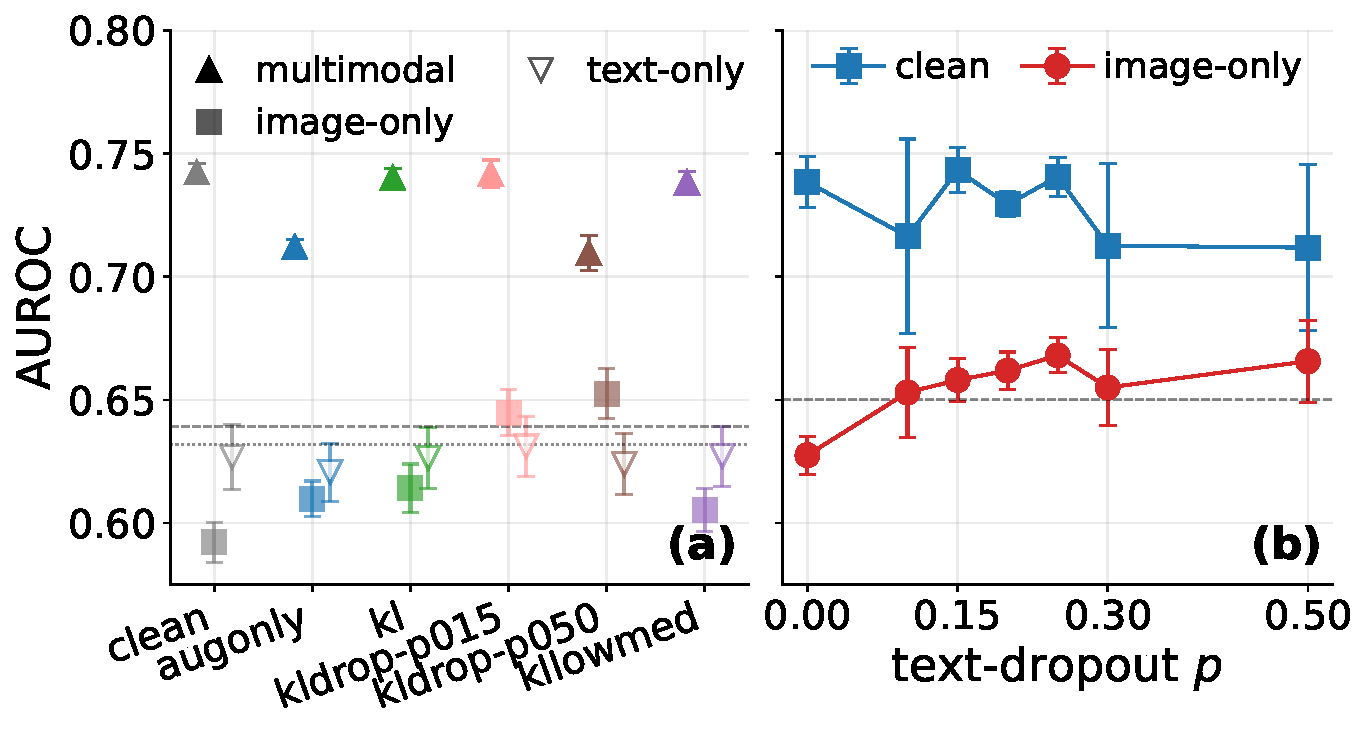
\includegraphics[width=\linewidth]{revival_and_sweep.pdf}
    \caption{\textbf{(a)} Per-branch forward AUROC (mean over $3$ splits
    $\times\,3$ seeds). \textbf{(b)} Dropout sweep (\texttt{test\_unseen}).}
    \label{fig:revival}
\end{figure}



\textbf{Why it works: a class-asymmetric false-positive veto.}
A per-example analysis on \texttt{test\_unseen} reveals the mechanism
(Fig.~\ref{fig:asym}): where \texttt{KLDrop-p015} and \texttt{KL} disagree, $97\%$
of \texttt{KLDrop}'s corrections are on benign memes (95\% CI $[94,99]$,
$n{=}131$) vs.\ $75\%$ on hateful memes for \texttt{KL}. The revived image branch
vetoes the text branch when an edited caption looks superficially hateful but the
image does not support it --- the over-moderation failure that erodes trust. The
choice is thus deployment-conditional: false-positive-sensitive contexts prefer
\texttt{KLDrop}, recall-sensitive ones prefer \texttt{KL}; the direction holds on
all three splits.

\begin{figure}[tb]
    \centering
    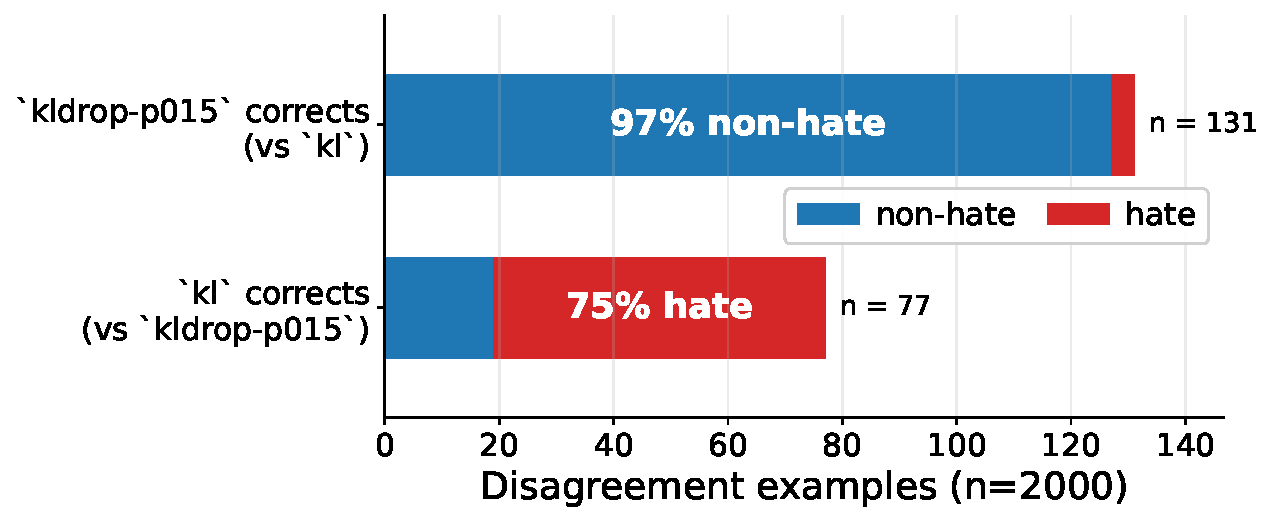
\includegraphics[width=\linewidth]{class_asymmetric.pdf}
    \caption{Per-example disagreements between \texttt{KLDrop-p015} and \texttt{KL}
    on \texttt{test\_unseen} ($n{=}2000$), split by gold label.}
    \label{fig:asym}
\end{figure}

\textbf{Adversarial Results.} Running adversarial PGD attacks on the CLIP model trained only on clean images collapses AUROC from $0.73$ to $<0.01$ (ASR $>0.98$) at $\epsilon{=}2/255$ and
to $0$ at $\epsilon\geq4/255$ (see Table \ref{tab:model_robustness}). 
Adversarial training restores PGD AUROC ($0\!\rightarrow\!0.61$ at $\epsilon{=}8/255$) at a clean-AUROC cost ($0.74\!\rightarrow\!0.62$) that stems from the adversarial objective; unfreezing the vision encoder is the near clean-free ingredient that makes this robustness genuine. Considering this white-box is unrealistic, the score is overwhelmingly positive. Other adversarial attacks such as gray-box or black-box will be much closer in performance to clean rather than white-box.


\begin{table}[tb]
\vskip -0.05in
\begin{center}\begin{small}
\setlength{\tabcolsep}{4pt}
\begin{tabular}{lccc}
\toprule
Model & Clean & Naturalistic & PGD \\
      & AUROC & AUROC ($\Delta$) & AUROC ($\Delta$) \\
\midrule
Clean                  & 0.738 & 0.598 ($-0.14$) & $<0.01$ ($-0.74$) \\
Naturalistic (p$0.15$) & \textbf{0.743} & \textbf{0.643} ($-0.10$) & $<0.01$ ($-0.74$) \\
Adversarial            & 0.616 & 0.540 ($-0.08$) & 0.610 ($-0.01$) \\
\textbf{Combined}      & 0.614 & 0.548 ($-0.07$) & \textbf{0.610} ($-0.00$) \\
\bottomrule
\end{tabular}
\vskip -0.08in
\caption{Worst-cell robustness on held-out \texttt{test\_unseen}
($3$-seed mean): clean AUROC, and attacked AUROC with the drop
$\Delta$AUROC vs.\ clean under the single most damaging naturalistic
perturbation and white-box PGD ($L_\infty$, $\epsilon{=}8/255$).
\texttt{KLDrop} (naturalistic, $p{=}0.15$) is naturalistically robust at no clean
cost but undefended against PGD; the combined model has the smallest degradation
on \emph{both} axes. The clean drop for \emph{Adversarial}/\emph{Combined} stems
from the multi-objective loss --- a frozen combined model shows the same
$\approx\!0.63$ clean --- not from unfreezing, which is near clean-free and is
what makes the PGD robustness genuine.}
\label{tab:model_robustness}
\end{small}\end{center}
\vskip -0.2in
\end{table}

\textbf{Combined model.} Naturalistic training alone still collapses under
white-box PGD (Table~\ref{tab:model_robustness}), so we unite both defenses in a
single model trained jointly on three views per batch --- clean,
naturalistic-perturbed, and PGD-adversarial --- under the composite loss
$\mathcal{L}_{\text{comb}}=\mathcal{L}_{\text{KL}}+\delta\,\text{BCE}(y,\ell_{\text{adv}})$
($\delta{=}1$, \texttt{KLDrop} text-dropout in the forward, $\ell_{\text{adv}}$ the
logit of the PGD view), unfreezing the vision encoder to absorb pixel-space
attacks. On held-out \texttt{test\_unseen} ($3$ seeds) it
inherits both: PGD AUROC at $\epsilon{=}8/255$ holds at $0.61$ (vs.\ $0.00$ for the
clean and naturalistic-only models) at the lowest naturalistic ASR ($0.09$),
trading clean AUROC ($0.61$ vs.\ $0.74$) --- a cost of the multi-objective loss,
not the unfrozen encoder (a frozen combined model shows the same clean AUROC, but
collapses under PGD). A single model can thus resist user obfuscation and
white-box attack at once.

\textbf{Applicability to other Datasets.} To validate our results further, we applied our training to MAMI, which showed very similar test results to the Facebook dataset. We also used our model to predict MultiOFF and results were also great.


\textbf{Limitations.}.

%%%%%%%%% ADD CONCLUSION SECTION %%%%%%%%%
\section{Conclusion}
\label{sec:conclusion}

A CLIP-fusion hateful meme detector is a text shortcut with a dead image branch
--- fragile to the text edits a real user applies, and undefended against
white-box PGD. Our recipe (KL consistency plus text-modality dropout) revives the
image branch above a dedicated baseline and raises held-out naturalistic
robustness by $76\%$ at zero clean-accuracy cost, acting as a class-asymmetric
false-positive veto for benign content; the white-box regime remains open for
adversarial training. Hateful meme detectors should thus be reported with a
modality-resolved robustness audit, not clean accuracy alone, since the dominant
failure --- over-flagging benign speech after a trivial edit --- is invisible on
clean benchmarks. These are research prototypes, not moderators; we release the
suite for defensive evaluation.

% \newpage


%%%%%%%%% REFERENCES SECTION %%%%%%%%%
\renewcommand{\bibfont}{\tiny}
\setlength{\bibsep}{0pt plus 0.2ex}
\bibliographystyle{IEEEtran}
\bibliography{main}



% %%%%%%%%% REFERENCES SECTION %%%%%%%%%
% \setlength{\bibsep}{0pt plus 0.2ex}
% \bibliographystyle{ieeetr}
% % This is the link to the refereces file.
% \bibliography{main}

\end{document}
